\documentclass[11pt,twoside,openright]{book}

\usepackage[papersize={120mm,200mm}, hmarginratio={3:2},bottom=0.8in,top=0.8in]{geometry}

\usepackage{times}
\usepackage[Lenny]{fncychap}
%\usepackage[Conny]{fncychap}

\usepackage[spanish]{babel}
\usepackage[utf8]{inputenc}
\usepackage[T1]{fontenc}

\newcommand{\personaje}{Nombre del personaje}

\usepackage{mathptmx}
\usepackage{etoolbox}

\usepackage[titles]{tocloft}

\usepackage{pdfpages}

\renewcommand{\cftchapleader}{\cftdotfill{\cftdotsep}}

% change the space before the titles
\makeatletter
\patchcmd{\@makechapterhead}{\vspace*{50\p@}}{\vspace*{0pt}}{}{}
\patchcmd{\@makeschapterhead}{\vspace*{50\p@}}{\vspace*{0pt}}{}{}
\makeatother

% change the space after the titles
\renewcommand{\DOTI}[1]{%
    \raggedright
    \CTV\FmTi{#1}\par\nobreak
    \vskip 10pt}% original: 40pt
\renewcommand{\DOTIS}[1]{%
    \raggedright
    \CTV\FmTi{#1}\par\nobreak
    \vskip 10pt}% original: 40pt


\title{Carne de los dioses}
\author{Juanjo Conti}
\date{}


% Evitar viudas y huérfanas
\widowpenalty=10000
\clubpenalty=10000

\begin{document}

\pagestyle{plain}

%IMPRENTA
%
\includepdf{empty.pdf}
%IMPRENTA
%
\includepdf{empty.pdf}

%\maketitle
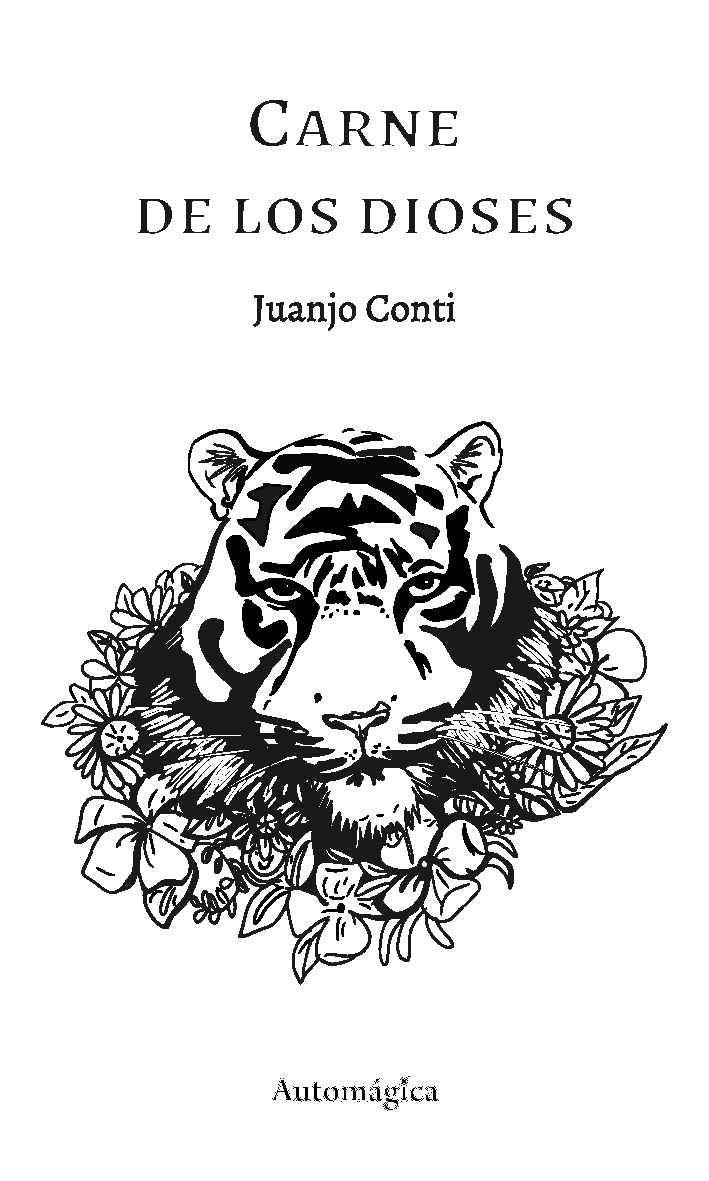
\includepdf{carne_de_los_dioses__bn.pdf}

%\cleardoublepage

\thispagestyle{empty}
\noindent
Edición automágica, 2016.\\

\vspace{0.5cm}

\noindent
\emph{Carne de los dioses} lleva la licencia
\emph{Creative Commons Attribution - NonCommercial - ShareAlike 4.0 Iternational}.
Esto significa que podés compartir esta obra y crear obras derivadas
mencionando al autor, pero no ha\-cer un uso comercial de ella.

\vfill

\noindent
%Más información sobre este libro:\\
http://www.juanjoconti.com/carne\\

\noindent
%Más libros del autor:\\
http://www.juanjoconti.com/libros

\cleardoublepage

\noindent
\begin{flushright}
\emph{
\emph{Carne de los dioses}\\
está dedicado a mis compañeros del taller\\
\emph{El brillo de la palabra},\\
testigos del nacimiento de muchos de estos cuentos.}
\end{flushright}

\cleardoublepage

\renewcommand*\contentsname{Índice}

\tableofcontents

\chapter*{Prólogo}

\begin{em} Armar un libro de cuentos es cansador y doloroso. Y no me refiero a
escribir los cuentos. Me refiero al trabajo posterior a esto.

Pasó un año o dos. Estuviste escribiendo. Asististe a un taller y cumpliste con
muchas de las consignas. Intentaste escribir una novela por tu cuenta, o dos, o
tres. Y llega el verano y, como además de escribir te gusta editar, te decís:
“Este verano imprimo un libro”.

Más o menos por el mismo tiempo, pero unos meses antes, te enteraste de un
concurso de cuentos. Tema: el agua. Hacés una búsqueda en tus archivos y
resulta que sí, que tenés un cuento, en el cual el agua, si bien no tiene un
papel principal, es el telón de la historia. \emph{Carne de los dioses}. Lo
escribiste hace ¿un año? como una broma para un grupo de amigos. Después le
recortaste las partes específicas y lo hiciste circular como un cuento más,
pero nunca lo imprimiste. Lo arreglás y lo mandás al concurso. No te gustan los
concursos por la burocracia que encierran: imprimir tres copias, enviarlas por
correo postal... Pero este es distinto. La entrega es por correo electrónico;
así que lo mandás. Una de las condiciones es que el cuento sea inédito. Este
seguro lo es... al menos, al momento de enviarlo.

Hay una imagen en el cuento que no recordabas, pero al releerlo, te impacta. Un
tigre. Un tigre con un collar de flores. Te gusta la imagen y le pedís a una
amiga que te haga un dibujo. Ella es tan amable que lo hace y el resultado es
genial. Tanto que te inspira a armar un libro de cuentos solo para que ese
dibujo esté en la tapa. El único problema es que el dibujo es en blanco y negro
y vos querés una tapa a color. La artista se niega a pintarlo, por lo que
decidís colorearlo por tu cuenta. Según tu esposa, parece pintado por un nene
de tres años, pero a vos te gusta. Le pedís a tu amigo diseñador que arme una
tapa con ese dibujo.

Después, llega  el momento de seleccionar los cuentos que integrarán el libro.
Reunís los textos; tu correctora amiga los corrige. Los mirás de un lado y del
otro. ¿Cómo agruparlos? ¿Cómo lograr un conjunto, un orden? Ninguna selección
reúne suficientes ejemplares. La de ribetes fantásticos tiene cinco textos. La
“costumbrista”, siete. Ensayás distintos índices; sacás, ponés, reordenás. Cada
vez que regenerás el libro, intentás mirarlo con ojos nuevos, pero no podés, ya
estás viciado.

Entonces, lo abandonás, lo dejás “macerar”. Te olvidás del proyecto por unas
semanas. Unas semanas que parecen meses. Luego volvés. Volvés y terminás el
trabajo. Te sentás en la silla y terminás el libro, porque yo quiero recibirlo
en mis manos.

\end{em}

\input{romantico.txt}

\input{amor.txt}

\input{guido.txt}

\input{carta.txt}

\input{explicacion.txt}

\input{carne.txt}

\input{dieta.txt}

\input{reyes.txt}

\input{lavalle.txt}

\input{matecocido.txt}

\input{fin.txt}

\input{restaurador.txt}

\input{vikingo.txt}

\input{dijkstra.txt}

%IMPRENTA

\includepdf{empty.pdf}

\end{document}
